%Tutkimusaineisto ja -menetelmät
% vai: multi-view stereo rig implementation
\section{3D scanning rig implementation}

\subsection{Functional specification} % {{{

Constraints on the rig were specified in loose terms, leaving much work on the background study.
Desirable properties of the system were given as:

\begin{itemize}
	\item Ease of use: the user should not need to know implementation details to acquire a 3D scan
	\item Portability: the system should not rely on affixing fixtures on the walls or the ceiling, for example
	\item Flexibility: for research purposes, many subjects should be possible to scan
	\item 3D and 4D: both static surface reconstruction and variations in geometry over time should be possible to scan
	\item Open design: by documenting the rig well and selecting readily available generic components, a similar system could be built if there was such a need, and the already built system could be extended
\end{itemize}

%There is a wide variety of different consumer grade digital cameras.
%Some of the main differences are dicussed below.

A general-purpose reconstruction rig has many practical matters to consider when comparing to the pure mathematical side.
A mobile rig should be light enough to carry and set up, but it should be rigid enough to give proper quality pictures and hold its calibrated configuration.
Distance to the photographed target should not be too short in order to not annoy human subjects, but a too large setup is difficult to build and needs lots of space.
Flexibility for arbitrary subjects means, among other interests, that the rig should be adjustable enough by means of camera positions and viewing directions.
When capturing video, the frames should be synchronized among cameras as described in \ref{sec:video}, which might not be perfectly possible with a reasonable budget.
Cameras must be chosen from a large selection of pocket cameras, system cameras, and industrial machine vision systems.

%- lens distortion?
%- rigid base, motion blur
%- baseline width, focus, depth, fstop etc
%- compression artifacts are nasty

% }}}

\subsection{Camera comparison} % {{{

Closeup subjects in the range of a metre or less introduce concerns in shallow depth of field, forcing the lens aperture small, and consequently, requiring bright lights or slow shutter speeds.
More sensitive sensor would require less light, but depth of field decreases as the sensor size increases.

As the capture environment will be a clean laboratory space and the cameras will mostly be controlled remotely, features usually important to photographers such as weatherproofing or user interface were not considered.

The section \ref{sec:cameratypes} presents in more detail the properties necessary for reconstruction.

Reliability on configurability and controllability was considered important.
Cheaper cameras fit more into a budget, offering more numerous content, but they might not be properly controllable.
External shutter release mechanisms have been researched more on DSLRs;
the manufacturers do not provide official specifications of the release connector pinouts, but they have been reverse-engineered for many models by individual tinkerers.

Zoom-only lenses, lack of raw processing, remote configuration and manual modes, and slower processing speed leave cheaper compact cameras out of the comparison practically altogether.
More expensive models do have comparable features, but their prices rise into the same range as with DSLRs that are more understood.

Canon DSLRs have been used previously on commercial setups [infiniterealities, ten24, capture lab likeness capture rig (ea sports/fifa), remedy].
Commercial video capture setups may use specialized machine vision devices and partly custom software to export data into suitable format.

Machine vision devices need several high performance computers for reliable multi-camera capture because of the lack of local storage.
While each camera outputs easily 1 Gbit/s of data or more (eq. \ref{gigabit-transfer}, one hard disk per camera is needed if the capture is long enough and does not fit in a computer's RAM, increasing the system cost and complexity.
Best mechanical hard disks currently have sequential write speed that just exceeds 1 Gbit/s;
newer solid-state disks (SSD) generally are two to four times faster.
For covering all the bandwidth, expansion cards would be needed per camera, count depending on the camera protocol.
Most PC motherboards can accommodate only a few cards, requiring several PCs.
Transfer speeds given by specifications and theoretical maximum frame rates for 12-bit raw full-HD frames are listed in table \ref{tab:busspeeds}; achievable rates would be less depending on bus overhead.

\begin{table}[h]
	\centering
	\begin{tabular}{l l l}
		Bus type & Maximum theoretical speed & Naive max.\ frame rate\\
		\hline \\
		USB 2.0 & 480 Mbit/s & TODO\\
		USB 3.0 & 3.2 Gbit/s & TODO\\
		Camera Link & 5.44 Gbit/s? & TODO\\
		FireWire & 3.2 Gbit/s? & TODO\\
		GigE & 1.0 Gbit/s & TODO\\
		SD card with UHS-I & 832 Mbit/s & TODO\\
	\end{tabular}
	\caption{Bus speeds and corresponding frame rates}
	\label{tab:busspeeds}
\end{table}

In detail, the camera properties that should be considered include:

\begin{itemize}
\item CMOS/CCD sensor. CMOS suffers from rolling shutter in video mode, while CCD is more expensive and rare.
\item Resolution and sensor size. Higher resolution covers more detail, until airy disk size is reached. Larger sensor is more sensitive to light and therefore results in lower noise.
\item Lens quality. High resolution is only useful if the lens is sharp enough, and color aberrations degrade image quality in general.
\item Dynamic range, i.e. bit depth of the processing pipeline. JPEG pictures have only 8 bits per color channel, whereas DSLRs and industrial cameras use more, often 12 to 14 bits per pixel (in raw format, that contains the color filter array effects before interpolation)
\item Continuous shooting rate. Controlled by many factors, the speed at which full-size pictures can be taken; on consumer cameras, image processing speed and memory card write speed have most effect, and on industrial cameras, the bus speed typically limits the rate.
\item Dust reduction. If enabled for some consumer cameras, it is implemented as high-frequency vibration of the sensor on camera bootup. Because it moves the sensor, affects calibration.
\item Optical stabilization works by moving a glass element inside the lens or the sensor itself, effectively moving the image on the sensor, having an effect on calibration.
\item Video frame rate, resolution, and compression. Cameras that support raw format usually only use raw for still pictures and compress the video, as raw video is unnecessary in the consumer market and uses lots of space. For image processing, each frame should be as little compressed as possible. Some DSLRs support writing only full keyframes instead of predicted frames, resulting in higher quality and file size.
\item For consumer cameras, USB read speed supported by the camera. Retrieving saved image or video data takes less time for faster interfaces.
\item External flashes. Practically all system cameras can be wired to an external flash unit; only some compact cameras support this. Industrial cameras are externally triggered and require custom wiring from the signal source.
\item Shutter lag. Lag measured between ordering the camera to take the picture to the actual moment where exposure starts should be consistent, and preferably small.
\item Weight and size. A smaller and lighter camera requires less bulky support structures.
\item Price. With a fixed budget, cheaper cameras can cover a larger area of the subject at a time because more cameras fit in the budget.
\item Availability. For an easily replicable system, it should be simple to purchase the hardware.
\item Configurability. Clearly, aperture, shutter speed and others should be manually controllable and repeatable without automatic features.
\item Low noise. Sensor noise shows immediately in the image quality, complicating correspondence and others.
\item Remote trigger. Practically all DSLRs have wired or wireless remote shutter releases; some machine vision cameras have optionally an external logic-level trigger input in addition to one that is set by the protocol in the data bus. Some protocols may have global commands to send throughout a group of cameras. (FireWire?) Otherwise, software trigger suffers from sporadic jitter from operating system and protocol non-determinism.
\end{itemize}

Prices for compact cameras that have the required features go up to the same price range as DSLRs or even higher, i.e. 500 EUR and up.

Having a much smaller production rate than larger manufacturers that target consumers (such as Canon or Nikon), industrial cameras have a broad price range from a few hundred euros to thousands, well correlated with pixel count and frame rate.
Lens prices for industrial C-mounts are moderate, at around 200-300 EUR.

% }}}

\subsection{Selected cameras} % {{{

A number of compacts, system cameras, and machine vision cameras were reviewed.
In this section, the selected key parts are described in detail.
Precise information on all hardware used can be found in appendix \ref{app:hardwareused}.

A DSLR is a good choice for still photos because of moderate price compared to image quality, and availability of usable software.
Video recording is notably worse than with machine vision that can produce higher resolution, raw data, and synchronized output;
because of a price difference of an order of magnitude, it was decided to leave high-performance video tracking as a minor feature.

Canon was chosen among others because of previously acquired knowledge of the manufacturer, previously proven work using the same maker [infiniterealities, ten24, capture lab likeness capture rig (ea sports/fifa example), remedy] and firmware customizability \cite{magiclantern}. % this also above in practicalities

\subsubsection{Canon EOS 700D DSLR}

\simplefig{h}{%
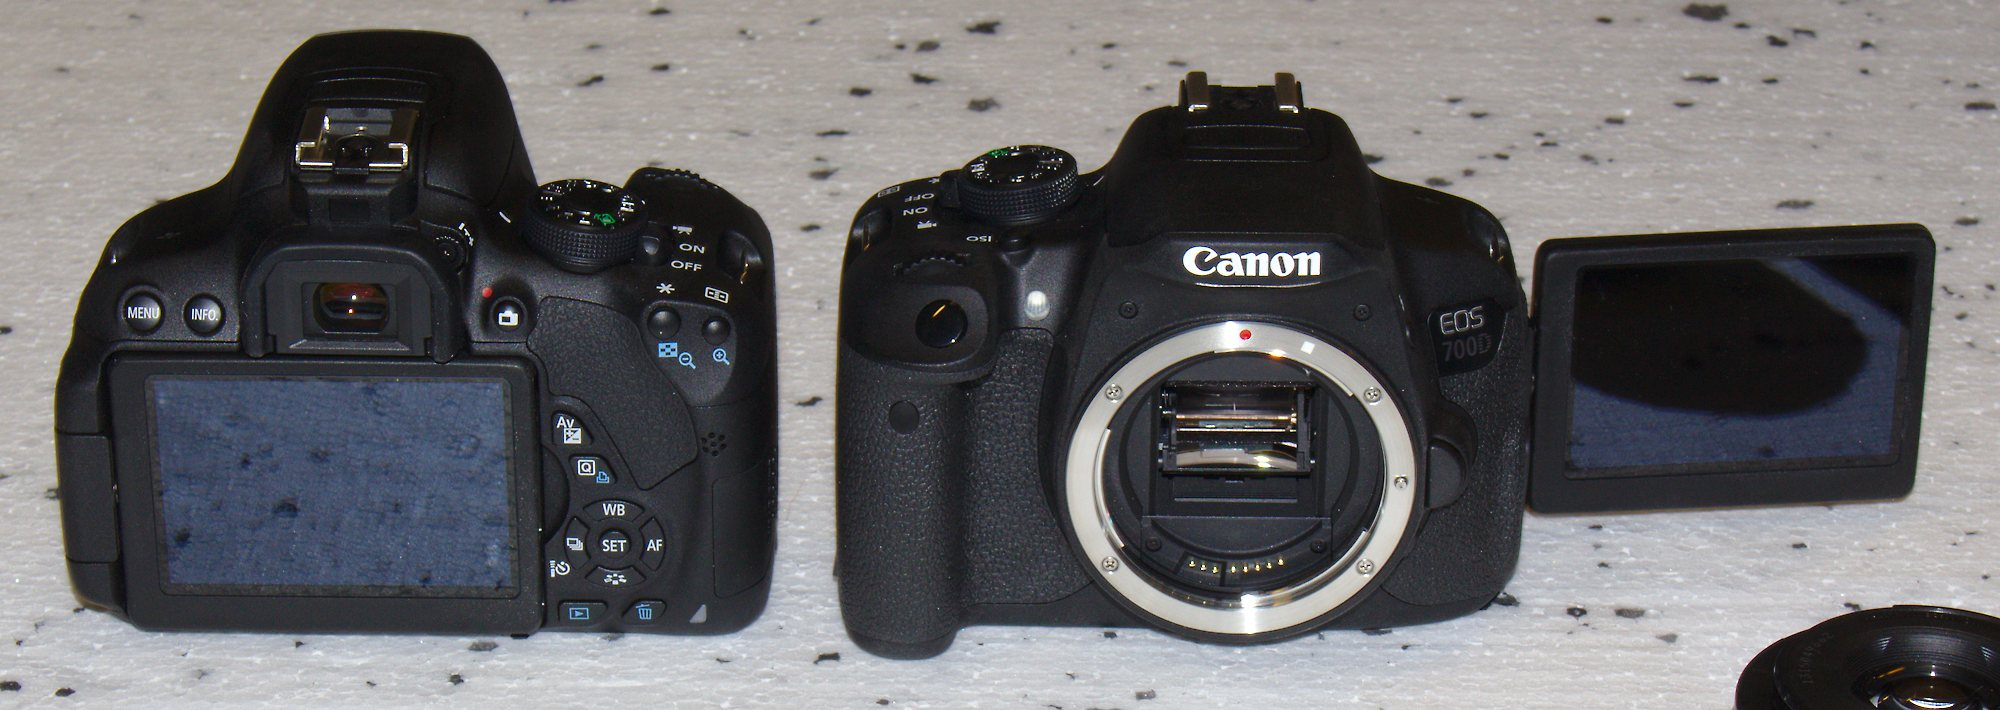
\includegraphics[width=0.4\textwidth]{eos700d}
}{fig:eos700d}
{Canon EOS 700D placeholder pic}

Canon EOS 700D body (or Rebel T5i in US), introduced in 2013, is among the newest of Canon's consumer range, with a price at about 600EUR.
Key features are shown in table \ref{tab:eos700dfeatures}.
A front view with a Canon 18-55 mm kit lens fitted is shown in figure \ref{fig:eos700d}.

\begin{table}[h]
	\centering
	\begin{tabular}{l l}
		Sensor type & CMOS\\
		Sensor size & APS-C 22.3 x 14.9 mm\\
		Pixel size & 4,3 x 4,3 $\text{\si\micro m}$\\
		CoC span at 0.019 mm & 4.4 pixels\\
		Image resolution & 5184 x 3456 pixels (17,9 million) \\
		Processor & Canon Digital Imaging Core (DIGIC) 5\\
		Bits per pixel & 14\\
		Shooting speed & 5 FPS\\
		Video mode & 1080p in 30 FPS or 720p in 60 FPS\\
		Write speed & $\approx$ 40 MB/s
	\end{tabular}
	\caption{Canon EOS 700D key features}
	\label{tab:eos700dfeatures}
\end{table}

Large pixel count combined to a good lens captures high-resolution detail.
The sensor's pixel size is not unnecessarily small but not as large as in full frame cameras.
Dynamic range with 14 bits per pixel is relatively large; most reconstruction programs use 8-bit images, though.
The 5 FPS continuous speed for full-size images can be used for testing high resolution motion, but the video abilities should be reasonable too.
Raw video recording is also possible with modified camera firmware, with reduced resolution limited by memory speed.

The sensor is labeled ``Hybrid CMOS'', a new Canon's technology that embeds phase-detection autofocus pixels in the sensor for fast continuous autofocusing in video mode.
A number of pixels is missing color sparsely around the middle of the sensor and are interpolated; they only introduce artifacts in raw video.

The camera also features a tilting LCD screen that has provided to be useful when looking the camera from the front.

Older models of the same product line can still be found in the market, such as 650D or 600D.
%700D has a newer processor and thus faster processing speed, faster memory card controller and others.
Resolution of the sensor has stayed same since 550D, introduced in 2010.
At the same time also cheaper new models are available, such as 1200D.
At a reduced price, less processing power is provided, resulting in slower operation but otherwise the cameras share mostly same features.
The more expensive professional cameras vary mostly by processing speed.

The camera uses Secure Digital (SD) memory cards for mass storage, supporting the UHS-I standard (Ultra High Speed).
Maximum write speed has been found experimentally to be approximately 40 MB/s.
A class 10 UHS-I memory card was selected; manufacturer claims 45 MB/s write speed.

Additionally, AC power adapters were chosen to operate the cameras without the need for charging batteries.
Canon sells adapters that plug in the camera's battery holder, providing continuous power at the expense of an additional cable per camera.

\subsubsection{Canon EF 50mm f/1.8 II}

Canon's EF-mount 50mm f/1.8 II lens (priced at about 110 EUR), shown in figure \ref{fig:canonef50mmlens} is well known for its excellent image quality at a low price.
The lens was introduced in 1990.
The 50 mm focal length provides good shooting distance for proposed subjects and is nearly distortion free.
Despite the poor plastic build quality, its glass is very good and it is well known as one of the best portrait lenses.
The lens changes between autofocus and manual focus modes with a mechanical switch, and the focus ring in manual focus mode is loose enough that it might need to be locked with tape if left on for a long time shooting to hold its position for a calibrated setup.

At a distance of one metre $d = 1 m$, the sensor size of $s_x$ x $s_y$ = 22.3 x 14.9 mm and $f = 50$ mm focal length, the area that fits in the frame is

\begin{align} \label{equ:areasize} \begin{split}
	a_x &= s_x * \frac{d}{f} = 22.3 \text{mm} * \frac{1 \text{m}}{50 \text{mm}} = 446 \text{mm}\\
	a_y &= s_y * \frac{d}{f} = 14.9 \text{mm} * \frac{1 \text{m}}{50 \text{mm}} = 298 \text{mm}
\end{split} \end{align}

which can be seen from similar triangles.
From eq. \ref{eq:dof}, the depth of field at this setting is about 16 cm for a f-number of f/11, or 20 cm for f/14, at circle of confusion of 0.019 mm, a reasonable depth for the given area size.

\simplefig{h}{%
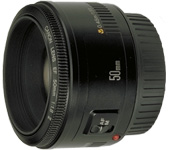
\includegraphics[width=0.4\textwidth]{canonef50mm-1}
%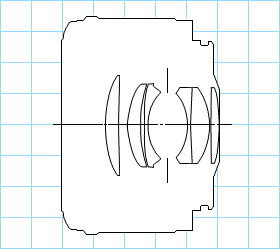
\includegraphics[width=0.4\textwidth]{canonef50mm-2}
}{fig:canonef50mmlens}
{Canon EF 50mm f/1.8 II, a fixed focus lens chosen for the rig (TODO replace pic)}

\subsubsection{Magic Lantern}

An important consideration was the ability to use the third-party Magic Lantern (ML) firmware add-on;
it was originally developed for tools and improved user interfaces for video recording, but has been extended for numerous other features too.
Firstly, it provides experimental support for raw video recording, easier remote triggering for video, and other hacks;
additionally, being open source, it can be modified for any custom purposes, such as multi-camera synchronization aids, if necessary.
It is a separate program that runs alongside the original firmware, using the same operating system and configuration menus.
A screenshot of a menu grid is shown in figure \ref{fig:ml-menu}.

ML is installed on a memory card, and it does not make permanent changes to the camera's original firmware.
Still, being third-party software based on reverse-engineering efforts, there is a small risk of unexpected instability.
ML has an active user forum, a wiki, and an automatic build system for nightly testing builds.
No stable release is offered for 700D yet, but the unofficial testing version has been long in use.
As an open source project, developed in a distributed fashion, it suffers from inconsistent documentation and is occasionally best examined by reading source code.

\simplegfx{h}{0.6\textwidth}{ml-menu}{
	Magic Lantern grid menu in movie mode.
}

% }}}

\subsection{Hardware construction} % {{{

\subsubsection{Mechanical choices}

With flexibility and mobility as requirements, the system should be built of removable parts that need no modifications to the environment, such as screwing bolts to nearby walls.
The separate parts should be small enough for transportation, but large enough for rigidity and build simplicity.
Each camera should be able to turn at least in landscape and portrait mode to fully utilize the frame for portrait subjects, such as human faces.

Two different major designs were considered: a frame consisting of industrial aluminium profile system, or individual tripod stands available in most photography stores meant for supporting lights.
For connecting the cameras, a custom profile could make use of also custom built parts; also, photography stores sell screws and clamps meant for connecting cameras, lights and other hardware.

Extruded aluminium profiles such as those by MiniTec, Item or Bosch Rexroth consist of square tube with a T-shaped slot running along each side for screws, sometimes called T-slot systems.
%The profile systems are commonly used in assembly lines and other automation installations in factories, but also in smaller assemblies
Mechanical dimensions vary by manufacturer but most supply a large catalog of connection brackets, hinges, screws etc.\ that allow much flexibility in the frame design.
A hobbyist-purposed manufacturer is OpenBuilds that targets open source projects, such as 3D printers and CNC routers.
The cost of such profile is around 10-20 EUR/m, with varying prices for connecting pieces; availability varies by supplier.

Ready-made light or speaker stands come in a variety of sizes and share a common design with an extendable center rod and three legs.
Typical light stands have an universal mount in top end of the rod for fastening a lamp.
Speaker stands do not share a similar standard; in general, they are also heavier and thicker to support a larger mass.
Most photography studio stores offer a variety of light stands; some have a similar range of speaker stands.

A custom aluminium profile system would have its benefits in rigidity and positional flexibility, because it could be built in any shape.
On the other hand, one rigid shape is more difficult to modify when such a change is needed.
Standard light or speaker stands are good because of their availability in normal stores.
They also can be moved around, which also means more work in configuring the camera poses again.
A stand consisting of mostly round rods lacks flat surfaces and slots that could be used for fastening parts together.
For that purpose, special clamps and ball heads are sold separately.

Machine vision cameras do not generally use same tripod screws aimed for consumer market, but are screwed on with custom bases.

\subsubsection{Selected design}

The selected method was to use ready-made, heavy duty lighting stands.
Millenium LST-310 (a brand by Thomann) is a sturdy three-legged lighting stand with a pole that can be zoomed several meters high.
Additionally, it has a rotating horizontal bar at the top.
Similar tripods were used in other projects in the same laboratory and they were found useful and rigid.
The relatively heavy weight (10 kg) makes the support structures steady. % FIXME weight
Four of these stands were bought, which should allow a moderate coverage around a subject. %and testing was done mostly with three, with three cameras in each.

For flexibility, each camera should be able to rotate in at least to horizontal or vertical pose, with arbitrary aiming position.
For that, Manfrotto 494 ball heads were used, connected to the tripod rod with Manfrotto 035 Super Clamps.
Figure \ref{fig:TODO} shows a complete connection from a stand pole to a camera.

The total structure of all nine cameras divided in three supports (figure \ref{fig:TODO}) takes up relatively little space, and is flexible enough to set up around any human-size subject or smaller.

Wires and power adapters are fastened to the stand legs in long-term use to reduce wires running on the floor.

% }}}

\subsection{Remote shutter synchronization} % {{{

For a rig with possibly non-static subjects but an intended result of a still frame, the cameras have to be synchronized to record the same data.
Photo synchronization was done with a remote mechanism provided by the camera, by driving the remote control of all cameras simultaneously.
In video recording mode, the same remote wire can be used with 3rd-party firmware to start recording.

% }}}

\subsubsection{Canon remote trigger} % {{{

The selected Canon EOS 700D has an input port for focus trigger and shutter release, in addition to the integrated focus and shutter button.
The camera uses a standard 2,5 mm stero jack for connecting external remote controllers.
Wired and wireless electronic remotes are available in the market, but no standard devices for triggering several cameras arbitrarily are well available. % seem to exist.
Fortunately, the triggering method is widely researched among hobbyists; it is well enough documented in the internet.

The remote release jack is a three-contact connector, where one pin serves as a common ground, and connecting another pin to the ground triggers the camera's autofocus and metering, and the third pin releases the shutter when connected to the ground.
Luk from doc-diy.net \cite{docdiy} describes the camera's trigger circuit internals; the wires supply some current that flows back to the camera via the ground pin, which is is safer to separate the cameras from each other electrically instead of connecting the similar remote wires of all cameras together.
A commonly used method among the DIY community is to use opto-isolators to control each camera individually, isolated from the shared control circuit.

An opto-isolator provides a galvanically separated switch that can be used to electrically ``connect'' the release wire to the camera's ground such that no electrical signal path is shared between the cameras.
The switch is a phototransistor that is triggered externally by the light transmitted from a LED.
Both the phototransistor and the LED are installed in a opaque plastic housing.
As an example, the opto-isolator device used in this work is shown in figure \ref{fig:singleopto} next to the circuit it was used with.
The particular device works in open collector setting, exposing the open collector pin and the emitter pin of the transistor.
Another common setting is a powered device that outputs a voltage signal from a power supply.

% TODO: fig:opto-isolator in physical form and in a schematic diagram next to each other

% }}}

\subsection{Synchronized multi-trigger implementation} % {{{

By connecting each camera to a separate opto-isolator and driving all of them from same source, all cameras are triggered simultaneously in a safe fashion.
To fully automate the system, the trigger device should be connected to the computer that downloads the photos from the cameras.
Additionally, the cameras are enabled to shoot separately in addition to the synchronized simultaneous mode.

\subsubsection{Platform}

In this work, a microcontroller prototyping platform called Nucleo-F401RE by STMicroelectronics was used.
This platform has a built-in USB port for simple communication.

A microcontroller (MCU) is a tiny computer in a single, usually fingernail-sized package containing a microprocessor core, RAM, program memory and peripheral devices; all parts required to run a single user-defined application typically with no general operating system.
The Arduino microcontroller board is another popular example.
The typical programming languages for microcontrollers are C and C++.
Communication on the other end of an USB connection can be implemented in any language.

A MCU was chosen over e.g.\ a computer-controlled relay board because of its customizability and low price.
On one hand, such a device is more complicated to set up than a simple switch, but on the other hand, it can be programmed to sequence the cameras in any arbitrary order.
It can also be used to measure the shutter delay and the actual precise time when each camera takes the picture; each has small unpredictable variations.
When capturing moving targets, measuring this lag variation could be of interest.

\subsubsection{Hardware}

\simplegfx{h}{0.6\textwidth}{nucleo}
{STM32 Nucleo-F401RE microcontroller development board.}

The Nucleo-F401RE (figure \ref{fig:nucleo}) is a prototyping board designed around the STM32F401RET6 microcontroller IC.
This MCU contains a relatively powerful 32-bit ARM core, space for 512 KB of program code, 96 KB of RAM, 51 general-purpose I/O pins available on the board, and other peripherals such as timers and analog/digital converters.

The trigger was constructed for ten cameras, functionally transferring trigger pulses from a PC to all cameras synchronously through opto-isolators and 2,5 mm stereo cables connecting to the cameras.
For each output, a Toshiba TLP621-2 dual opto-isolator was used, mainly because they were readily available; any similar device would work.
An output pin in the microcontroller drives an LED of the isolator, making the corresponding transistor conductive.
Schematic of one camera controller is shown in figure \ref{fig:singleopto}.
Each LED is driven through a current-limiting resistor of 220 ohms, resulting in about 10 milliamps of LED current with the LED voltage drop of 1.15 V specified by Toshiba datasheet, matching the specified test condition.
This results in tens of milliamps of maximum available collector current, which is orders of magnitude more than that of supplied by the camera. % TODO write this better
The cameras have shown to consistently respond to this signal well.

The circuit was initially constructed on a solderless protoboard, ``breadboard'', shown in figure \ref{fig:camsremote-proto}.
After proving that the circuit worked, a proper circuit board was built and installed in an extruded metal enclosure.
Board layout is shown in figure \ref{fig:triggerboard} and the built case without final lid in figure \ref{fig:camsremote}.
Full schematic for the whole circuit is available in the appendix \ref{app:fullschematic}.
The circuit was drawn with the Cadsoft EAGLE, a pcb design software; complete schematic and layout files are available in \url { http://github.com/sooda/TODO-URL-HERE }.

The circuit board was designed to fit in a recycled enclosure that has inside dimensions of 5 by 3.9 inches (127 by 99 mm).
The used housing has a removable lid, but any box with a height of 1.4 inches (35 mm) or more should fit.

%\simplegfx{p}{0.8\textwidth}{singleopto} % TODO: disconnect ground from the camera side
\simplefig{h}{%
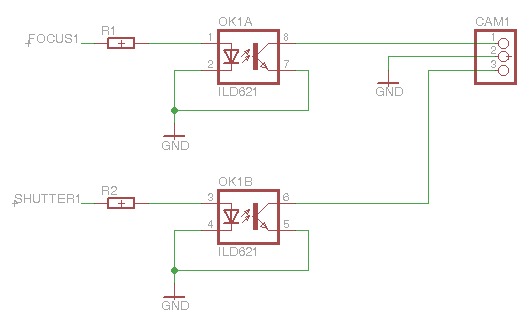
\includegraphics[width=0.5\textwidth]{singleopto}
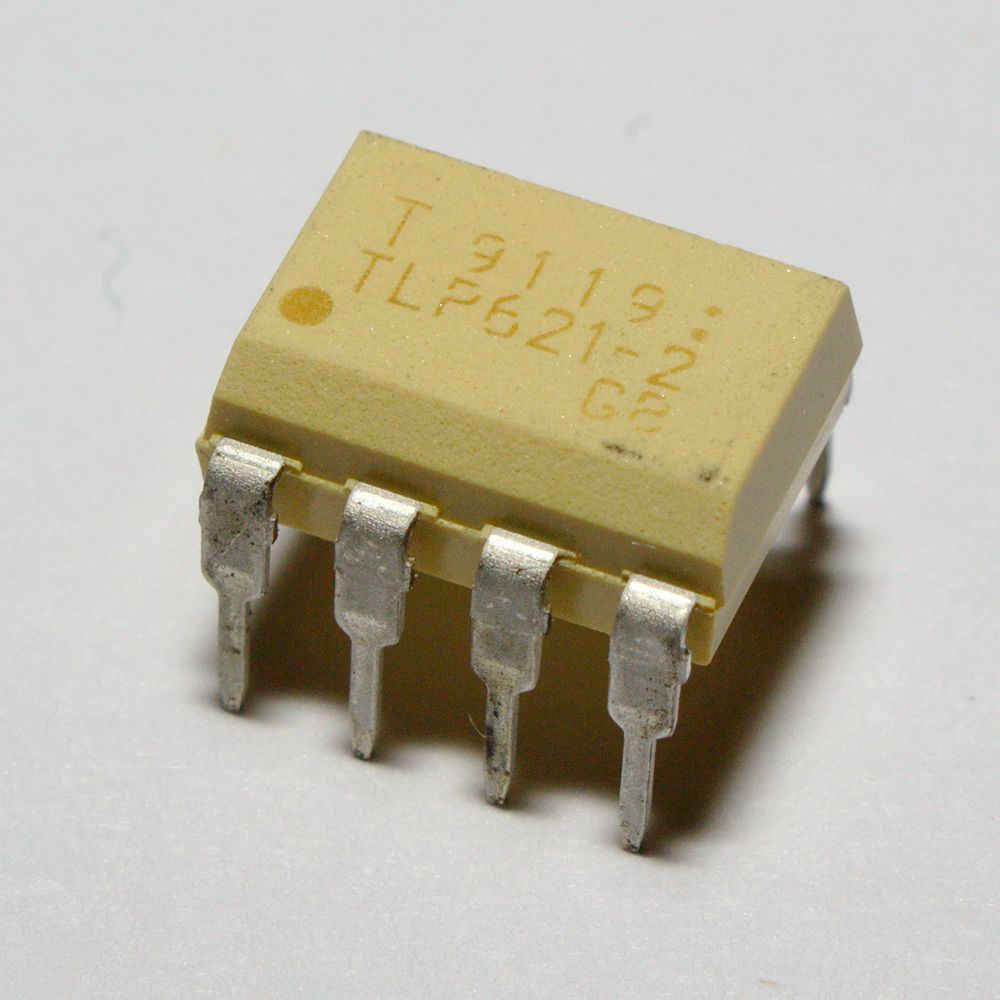
\includegraphics[width=0.3\textwidth]{tlp621-2}
}{fig:singleopto}{
	Left: a single opto-isolator pair for shutter and focus of a camera, including the current-limiting resistors and a pin header connector for the camera signals.
	Right: TLP621-2 dual opto-isolator in a DIP8 through-hole package, with physical dimensions of approximately 10 by 7 mm.
}

\simplegfx{p}{0.8\textwidth}{triggerboard}
{Printed circuit board layout for the trigger box. Full schematic available in the appendix. \ref{app:fullschematic}}

\simplegfx{p}{0.8\textwidth}{camsremote-proto}
{Remote trigger tool prototype on a solderless breadboard.}

\simplegfx{p}{0.8\textwidth}{camsremote}
{Remote trigger tool in a case, with lid removed. TODO better pic.}

\subsubsection{Code}

STMicroelectronics advertises the Mbed programming environment and library for the board as an option for writing software for the MCU.
The toolchain that compiles the binary for the board works also via the browser in a cloud service, but the libraries can be also installed locally.
All MCU-side code was developed using the Mbed libraries, built locally with the GCC-ARM Embedded toolchain \cite{launchpad-gcc-arm}.
Mbed hides the hardware complexity of the platform, making the total application source code size small (less than 200 lines of C++).

The MCU software, or \emph{firmware}, communicates via a serial line that the board passes through USB as a standard virtual serial port (``usb tty'' in Linux or ``COM'' port in Windows terminology), requiring no special drivers.
Communication protocol consists of flags for setting focus or shutter mode and entering bit flags that describe what cameras should be affected, in text mode.
The device echoes the sent characters back, making it easy to test with a serial console.
The protocol is described in detail in table \ref{tab:triggerprotocol}.

The code also monitors a the Nucleo's integrated button that can be used to focus and trigger all cameras simultaneously.
One press focuses all cameras, and subsequent presses send a short shutter press.
The reset button resets the whole microcontroller, restarting the program with no focus or shutter signals selected.

\begin{table}[h]
	\centering
	\begin{tabular}{l l}
		Set focus pin state & Fxxxxxxxxxx\\
		Set shutter pin state & Sxxxxxxxxxx\\
		Reset all to unpressed & R\\
		Example: press focus on first and third & F101\\
	\end{tabular}
	\caption{
		Remote trigger protocol; the letter x signifies a single bit (digit 0 or 1) and can be omitted from the start, in which case it is assumed 0.
		Note that the messages set the whole button state instead of sending ``keypresses'';
		to emulate a full keypress, the state must be set to 1 followed by a 0.
		Each command must be finished with a space or newline character.
	}
	\label{tab:triggerprotocol}
\end{table}

The used Mbed library does not actually turn all pins on at exactly the same time but in fast succession.
This is not a problem because of the high clock speed of the processor;
the difference between first and last pin changes was measured to be a negligible 1,6 microseconds.
%Expected variance from each camera is supposed to be orders of magnitude longer.

Control software for the host PC was implemented as a small command-line Python script communicating to the virtual serial port of the Nucleo board.
The host controls the trigger's outputs individually, normally driving all the outputs at once.
Sequential or other forms of triggering are possible, because the cameras are controlled individually in hardware.
For example, as each camera is able to record five full-resolution frames per second in burst, interleaving the nine cameras results in short 45 FPS full-resolution imagery.
Also, when using the internal pop-up flashes in the cameras, they can be fired separately to circumvent issues in lighting synchronization or exposure control.

The same MCU can be reprogrammed with another firmware at any time; it was used also for measuring shutter delay of one camera, see section \ref{sec:shutterdelaymeas}.

The programs are available in \url { http://github.com/sooda/TODO-URL-HERE } with source code.

% }}}

\subsection{Custom camera control software} % {{{

% breeze systems $129 per cam
% smartshooter

% FIXME clumsy
% esper design etc.
%General parallelized image acquisition from a large set of cameras has not yet established such a state that general purpose software would be easily available.
%Commercial solutions probably exist, but they are often strictly bound to a specific hardware, expensive, and inflexible.

Some custom techniques were used to preview images of all cameras simultaneously, configure the settings of each in parallel, and retrieve the captured images from them in order.

Like the MCU board layout and firmware, all programs and their sources can be downloaded from \url { http://github.com/sooda/TODO-URL-HERE }.

% }}}

\subsubsection{Camera control library} % {{{

gphoto2 \cite{gphoto2} is a well-known free and open-source application and library in the C programming language for controlling digital cameras on Unix-like operating systems, supporting over a thousand cameras.
The software consists of a command-line control tool of the same name, \emph{gphoto2}, and a library API, \emph{libgphoto2}.

Instead of relying on each camera manufacturer separately for a software development kit, gphoto2 abstracts common operations behind the same interface.
For example, Canon and Nikon, some of the biggest camera manufacturers, both provide SDKs for controlling their devices remotely via a USB connection from Windows and Mac OS X. \cite{canonsdk} \cite{nikonsdk}
Sony provides an SDK for Android and iOS. \cite{sonysdk}
Olympus has had an SDK, but it is no longer available. \cite{olympussdk}
To support all vendors, one would have to write code for all APIs.
In addition, development kits provided by the vendors may be more restrictive and may not be fully available.
%Canon provides a Digital Imaging Developer Programme that requires registration to be able to download the SDK (EOS Digital SDK, or EDSDK).

Furthermore, the Canon EDSDK claims in the manual not to support sessions to more than one camera in parallel.
This technical issue could probably be overcome with additional work, though.

Libgphoto2 implements the \emph{Picture Transfer Protocol (PTP)} \cite{ptpTODO} for setting properties and transferring pictures.
Details on list of configurable properties and sequences for capturing pictures and preview vary among manufacturers, and the library has most thorough support for Canon and Nikon cameras.

A ``wrapper'' code was written in C++ for libgphoto2 to automate memory and resource management and to write the programs themselves in clean C++; libgphoto2 itself is implemented in the C language.
Libgphoto2 exposes the data as objects, and the wrapper simplifies their handling and implements some more complicated operations, such as creating a new camera object, and downloading preview frames and actual shots.
The library itself is also not thread-safe: if a camera is used in to threads of execution simultaneously, unexpected errors happen.
Locking mechanisms were written for the wrapper to prevent more than one executing threads from accessing a camera instance simultaneously.
The library initialization was also protected, because it loads camera-specific sub-libraries only after first use; if many cameras are tried to initialise at the same time, another error would occur.

The wrapper is written for exclusively libgphoto2 in mind, but as it actually hides the implementation details strongly, it could be ported to use e.g. EDSDK behind the scenes without affecting the actual applications using it.

% }}}

\subsubsection{Previewing} % {{{

\simplegfx{h}{1.0\textwidth}{gphotogrid}
{A custom written program for displaying a preview feed of many cameras in a grid and configuring exposure time, aperture, and sensitivity. (TODO update later with the finished one)}

%\simplegfx{h}{1.0\textwidth}{gphotogridtimeline}
%{TODO}

Although each camera can be positioned by individually looking through the viewfinders, a simple preview live feed is almost mandatory to properly set up a new configuration to see the big picture.
A preview matrix of all cameras makes it easy to identify the cameras and to see if they all have been pointed to correct directions, and to verify that their settings are the same by judging from the image quality.
The program is shown in figure \ref{fig:gphotogrid} and is found in the github repository under the name \emph{gphotogrid}.
It is written in C++ and uses the libgphoto2 wrapper for camera control and the wxWidgets GUI library for the user interface.

Libgphoto2 provides an interface for reading a camera preview frame at a rate of several frames per second, speed depending on the number of cameras used in parallel because of USB bus limits and CPU processing power as the images are resized to the screen.
A preview feed is connected to each camera to download the frames as fast as possible, and the user interface displays them as a grid, with configurable camera order.
Because libgphoto2 does not offer asynchronous image or configuration transfers, a new thread of execution is set up for each camera, and the preview pictures are transferred to the main screen via concurrency-safe queues in the application itself.

A timeline widget was also developed to investigate the points in time when the preview frames have been grabbed, in the hope of synchronization.
Observing the times was found to be of no use, because the pipeline from camera to application seems to be so complex that the preview frame rate is completely sporadic, with no ability to control the frame order or timing.
The application includes a checkbox for ``synchronizing'' the preview grabber threads so that no camera starts to read a new preview before all have read the last frame; this seems to have no noticeable effect.
The timeline is depicted in fig. \ref{fig:gphotogridtimeline} (TODO).

It is recommended to spread the cameras as evenly to all USB root hubs as possible to help even out the transmission capacity, maximizing the frame rate.
The same is recommended when downloading the actual images.
The USB hub where a device is connected can be verified in Linux by looking at the output of the \emph{lsusb} command-line tool.

The cameras are identified and ordered by a name written to the configuration set under a property called \emph{artist}, found at least in Canon DSLRs.
The artist name can be set either via USB or from the camera's physical user interface, and it is supposedly originally meant for writing the camera owner's name in the image file's metadata, along with copyright information.
For the camera rig, a single letter was used for each camera, ordered from \emph{A} to \emph{I}.
A separate configuration property stored in the camera itself is most robust; USB port name can be used as an alternative to identify the cameras, but the port name changes when the cameras are plugged in another way when rebuilding the rig or using another computer.

% }}}

\subsubsection{Configuration} % {{{

Remote control of all cameras is required to set all settings, such as shutter speed, jointly from the same computer instead of clicking on each camera's buttons manually.
The preview matrix program allows to to change exposure time, aperture size and ISO sensitivity, but more tools were written for automatic configuration.

Other small command-line scripts were written using the gphoto2 command-line tool:

\begin{itemize}
	\item \emph{config}: reset common parameters to defaults for all cameras, listed in the script itself
	\item \emph{forall}: run gphoto2 with the user supplied arguments for all cameras serially
	\item \emph{forallp}: as forall, but in parallel, saving time
	\item \emph{post-download-by-camid}: download all previously shot files stored in the cameras to directories named by camera artist name
	\item \emph{readconfig}: read and copy settings from one camera to all others currently connected
	\item \emph{release-uilock}: unlock the physical user interface of connected cameras by fetching a listing the filesystem; a workaround for the Canon glitch described below
\end{itemize}

The \emph{forall} and \emph{forallp} scripts are trivial shortcuts to autodetecting all cameras and proxying commands to gphoto2 for each, and is useful for case-specific problems or e.g. setting individual configurations temporarily.

With \emph{readconfig}, one camera can be configured manually with trial and error, and the settings can be cloned to others automatically.
Testing the parameters on a camera manually is more convenient in some cases.

Either libgphoto2 or the EOS 700D camera has a bug that locks the camera's physical user interface when configuring the cameras and even quitting the program:
it appears that this is a safety feature that is left on and probably gphoto2 does not release it properly.
When setting or getting any configuration, the camera screen turns off and all buttons stop responding until the camera is rebooted, USB cable is unplugged, or if gphoto2 touches the camera's filesystem.
Listing the files is thus enough and it has no side effects, and a workaround script was written to perform it for all connected cameras.

% }}}

\subsubsection{Image acquisition} % {{{

% offloading

A command-line tool called \emph{paraphotos} for downloading the images in realtime in parallel from each camera was developed in C++ using the same libgphoto2 library wrapper.
The cameras send a notification when a new photo is taken with the shutter button or the remote release.
When this new file is found, it is downloaded and named by a running index and camera name.
The user is notified when all cameras have finished for a single shoot; also, when the program is requested to quit, it first waits until the last pending download is finished.
Each download task runs in a separate thread of execution to overcome the synchronous nature of libgphoto2, as well as the notifying task; figure \ref{fig:img-get-process} shows simplified code control flow.

\simplegfx{h}{0.8\textwidth}{img-get-process}
{FIXME: this is ugly. Simplified flow graph of the paraphotos program control flow.}

Almost the same functionality could have have been achieved with the gphoto2 command-line utility; using the library directly with C++ resulted in cleaner code and probably faster operation.

Video acquisition is not possible in realtime; instead, the video files have to be saved on the memory cards first, and downloaded when the recording is complete.
The \emph{post-download-by-camid} clones the file systems from the cameras to local disk, bringing the video files accessible.

Video format should be set to 720p at 50 or 60 FPS or 1080p at 25 or 30 FPS.
Both resolutions result in a video bitrate of approximately 5 MB/s with default settings.
The video format is H.264 encoded in a Quicktime MOV file, with a stereo audio in raw lossless (PCM) format with 48 kHz sample rate and 16 bits per sample.

The bitrate can be extended from Magic Lantern's menus, but bitrate changes are still experimental code and recording may stop if the camera or the memory card is not fast enough.
Video keyframe rate can also be changed with a development version of ML and probably will be stable in the future;
in the video codec used, the frames can be \emph{I-frames} (intra-frames), with fully encoded data, or \emph{predicted frames}, encoding changes between frames, with less accurate information.

% }}}

\subsection{3D reconstruction software survey} % {{{

When the imagery has been downloaded to a PC, the actual reconstruction can be started.
There is a wide collection of libraries, open-source tools and commercial packages for both automatic reconstruction and generic mesh editing for post-processing the data.
 % }}}

\subsubsection{Free libraries} % {{{

There exist several generic computer vision and geometry processing libraries, most common of them being probably OpenCV \cite{opencv}, Point Cloud Library (PCL) \cite{pcl} and Computational Geometry Algorithms Library (CGAL) \cite{cgal}. These are written in the C and C++ languages and they have bindings to several scripting languages too.

OpenCV contains a large set of tools for 2D image processing and extends also to camera calibration and 3D reprojection.
It is probably the most commonly known and most used computer vision algorithm package.

PCL contains a set of algorithms for filtering, segmentation, registration, visualization, and more for working on data sets that consist of points that may share attributes such as colors and normals. CGAL's scope is in the same field, concentrating on a little more advanced topics.

% }}}

\subsubsection{Free programs} % {{{

While libraries can be used to write new tools, many pieces of software are readily available that implement the algorithms presented and are distributed in source code form and/or readily usable binary executables.

Camera Calibration Toolbox for Matlab, also included in OpenCV as a C port, is a more or less standard tool to single-camera and stereo camera calibration.
The toolbox computes undistortion maps and intrinsic and extrinsic parameters with checkerboard images using non-linear optimization and homographies. \cite{camcalmatlab}

Bundler is a bundle adjustment and structure-from-motion system for computing camera poses and sparse point clouds. \cite{snavely2006photo}

SiftGPU, a SIFT implementation for graphics processing units. \cite{changchang2007siftgpu} It is built on Sift++ \cite{vedaldi2011sift++}; both are based on difference of gaussians, a method for edge detection \cite{marr1980theory}

Multicore (parallel) bundle adjustment: PBA computes the bundle step in a way that exploits the modern parallel nature of computer processors that have several computing cores. \cite{wu2011multicore}

Patch-based, clustering multi-view stereopsis (PMVS/CMVS) starts from a set of matching keypoints (features) and expands them to a dense patch set iteratively. \cite{furukawa2010accurate,furukawa2012patch}

VisualSFM \cite{wu2013towards} is a common and free but closed-source integration tool simplifying the workflow using external programs.

Meshlab \cite{meshlab} is a portable editor of point clouds and meshes.
It can be used interactively and scripted to do the same steps automatically.
In a reconstruction pipeline, it is one of the last processing steps, used for removing outliers or fitting a surface on a point cloud with the poisson surface reconstruction method, and finally projecting the textures to the generated mesh when given the camera parameters in relation to the point cloud pose.
It can also perform registration between point clouds.

Screened poisson surface reconstruction, or PoissonRecon, is another stand-alone program as an alternative for surface fitting. \cite{kazhdan2013screened}

Cmpmvs is a multi-view reconstruction software for transforming a set of calibrated image data to a full textured mesh, used in a similar way as VisualSFM but using internally a different method based on graph cuts and weakly-supported surfaces.
\cite{jancosek2011multi}

Python Photogrammetry Toolbox is another pipeline combinator for full 3D reconstruction, popular in archaeological fields. It combines Bundler and PMVS and others. \cite{moulon2011python}

SFM toolkit combines Bundler and CMVS/PMVS.

VisualSFM is probably the most common tool in the open source community.
It integrates into a few clicks the pipeline from images to 3D point cloud, using SiftGPU for features, PBA for camera estimation, and PMVS/CMVS for dense matching.
A common post step is to use Meshlab to filter outliers away from the data and to build a triangular textured mesh of it with the input points and normals.

%(VisualSFM screenshot here)

% }}}

\subsubsection{Commercial solutions} % {{{

There is a large selection of commercial software available, often accompanied with a 3D scanner.
Some companies offer completely specialized rigs, some sell a scanning device and a general-purpose software alongside it which can be used as standalone and some only sell software, leaving the hardware implementation to the user.
Examples include:
% FIXME emphasis on differences

\begin{description}
	\item[Autodesk 123D Catch] is a free web-based application for automatic structureless reconstruction.
	\item[Agisoft PhotoScan] has two editions, for 3D designers and professional geographic content manipulation; among the geographic features, it is very suitable for multi-view reconstruction in content generation, and has an active forum for its users.
	\item[CaptiveMotion] provides a facial capture and retargeting system that can be used with full-body mocap.
	\item[MotionScan] is the technology behind the video game L.A. Noire. \cite{rockstar2011noire} It uses tens of cameras to recover detailed structure.
	\item[Faceshift] encodes a markerless face captuer in a feature space that describes virtual muscle and bone movements.
	\item[3DF Zephyr Pro] is another automatic photo reconstruction system.
	\item[Mova Contour Reality Capture] does high-performance surface capture with a large array of cameras.
	\item[Pendulum Studio] provides a capture system called Alter Ego that integrates with game engines.
	\item[Pix4dMapper] converts aerial images to geometric surface models.
	\item[Acute3d] is targeted for large-scale photogrammetry and cultural heritage digitization.
	\item [FARO] manufactures hardware and provides scanning software for 3D documentataion and surveying, and provides a free application for Kinect-based scanning
	\item[Trimensional] is a 3D scanner for iPhone
	\item[Fuel3D] is a complete handheld scanning system
	\item[Dimensional Imaging ltd.] provides DI3D and DI4D systems for static and dynamic surface capture, respectively.
	%\item[SynthEyes] 
	\item[Pixel Farm] provides tools for CG integration and match moving.
	\item[3D-equalizer] is a multi-platform 3D tracking solution for the visual effects industry
	\item[Smart3DCapture] targets GIS and large-scale reconstruction.
	\item[V-STARS] by Geodetic System has emphasis on 3D measurement and engineering.
\end{description}

% TODO vicon; bradley face capture explains some.

%\subsubsection{Other}

(TODO)

%- voodoo camera tracker
% cyberware no longer exists, was used in films in hollywood
%- canoma no longer
%- bundler based on photosynth?
%- janimation head tech
% - KLT: http://www.inf.ethz.ch/personal/chzach/opensource.html
% http://slowmovideo.granjow.net/

% }}}

\subsection{Sample reconstruction pipeline} % {{{
%\subsection{Full reconstruction} % {{

Both shape and texture are considered in this work. Only diffuse color (albedo) is of interest; more complex material properties are assumed to be captured in other means and not spatially varying.

Basic uv mapping. Project texture to computed mesh. Somehow use colors and optical flow everywhere...

Postprocessing: remodel the mesh (face), see what it would look like. Refine parameters to get a similar output as in the photos (normal map etc.), backproject. Use colors and highpass them; assume uniform lighting and locally uniform texture color (bradley). (Simply a rendering technique, that level of detail in 3D structure might not be needed).

facial expression space, faceshift, face muscles
%
%KINECT 2 HYBRID SHIT YEA
%
%eigenface / pca / AAM model (?)
%
%poisson surface vs ball pivoting
%
%visual convex hull, bbox for constraining

% }}}

\subsection{Computer requirements} % {{{

any pc with usb and linux/mac/?? will do, the bigger the better

% }}}

